\clearpage\subsection*{3−1 CGIについて勉強しよう}
\refstepcounter{PagePtr}\label{P:CGI}
ここではCGIについて勉強しよう。第1回で作成したwebページはいわば静的なページです。静的なページとは、常に同じ画面を表示するページのことです。ですが、CGI(Common
Gateway
Interface)を用いることによって動きのあるページ、動的なページを作成することができます。動的なページとは表示させるたびに違う画面を表示することができるページのことです。アクセスカウンターはたまにwebページについていることがあります。アクセスカウンタというのは、そのwebページに今までどれぐらいの人がアクセス(接続)したのかを表示させるものです。webページにアクセスするたびにアクセスカウンタの数は\ruby{増}{ふ}えていき、毎回同じ数字にはなりません。これはアクセスするというアクションによってページに変化を起こしているのです。さらにCGIを用いることによって以下の機能を作成することができます。


\bigskip


\centering
\label{P:slide_p28}
\begin{minipage}{\textwidth}
          \begin{minipage}{0.45\textwidth}
	   \textbf{・アクセスカウンター}\\
	   \centering
            {\upshape
              \centering
              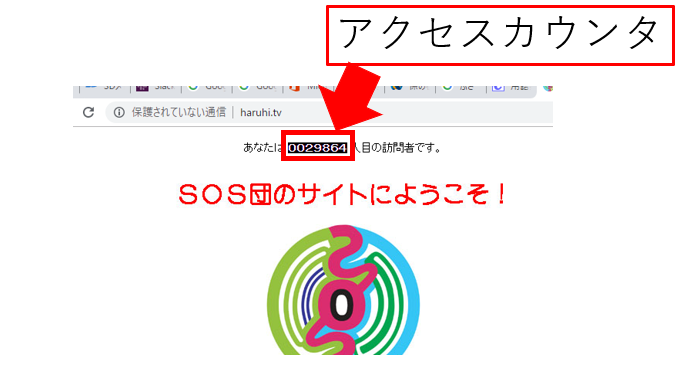
\includegraphics[width=0.8\linewidth]{text07-img/ome7-img046.png}}
          \end{minipage}
          \begin{minipage}{0.45\textwidth}
	   \textbf{・アンケートフォーム}\\
	   \centering
            {\upshape
              \centering
              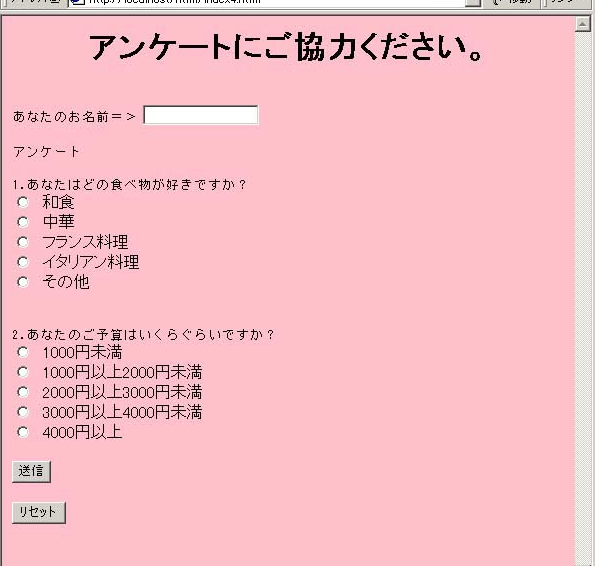
\includegraphics[width=0.8\linewidth]{text07-img/ome7-img047.png}}
            \end{minipage}
\end{minipage}
\flushleft


\bigskip

{\bfseries

	・\ruby{掲示板}{けいじばん}}



\centering
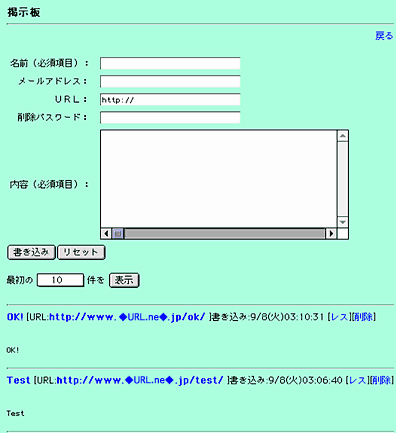
\includegraphics[width=4.431cm]{text07-img/ome7-img048.png}
\flushleft





\bigskip

みんなが作ったwebページやほかの静的なページはどのようなやり取りで表示させているか見ていきましょう。次の図を見てください。

\bigskip

\clearpage


\centering
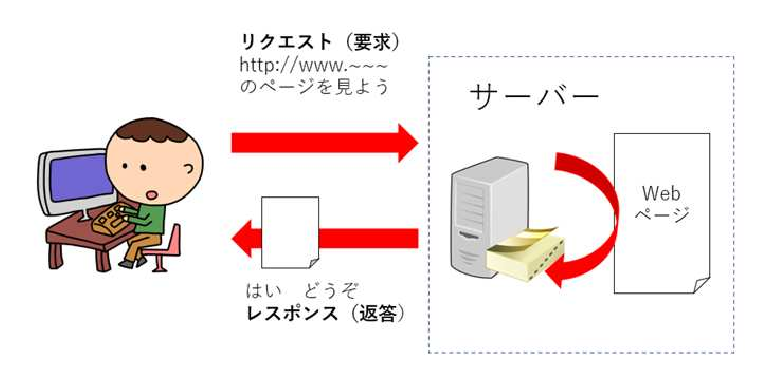
\includegraphics[width=0.75\textwidth]{text07-img/ome7-img049}
\flushleft


webブラウザで検索したりしてwebページを表示させることをリクエスト(要求)といい、そのリクエストを受け取ったそのwebページのあるサーバーが要求したところにレスポンス(返答)を返します。要求されたら返すのみで、webページに変化はなく同じものを見せていました。ですが次の画像をみてください。


\bigskip

\centering
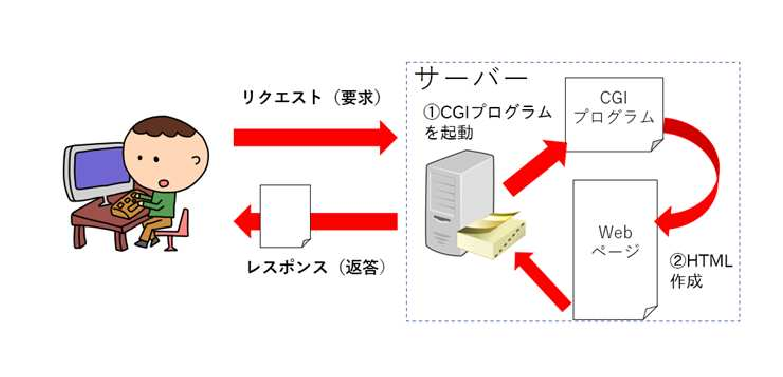
\includegraphics[width=0.75\textwidth]{text07-img/ome7-img050}
\flushleft


CGIを使った動的ページでは、サーバーが皆さんからwebページを要求されるたびに、CGIプログラムで新しいHTMLを生成しています。それにより、毎回違うwebページを見せることが可能なのです。この教科書では皆さんのラズベリーパイと今までの講義で学んだことを生かしたCGIを体験していきます。


\bigskip

\refstepcounter{Question}\theQuestion 動的なページとはどのようなものでしょうか。また、動的なページを作成する場合に用いるものは何でしょう。\label{Q:dynamicPage}\\

% 問題7-9  
% 動的なページとはどのようなものでしょうか。また、動的なページを作成する場合に用いるものは何でしょう。


  

  

  

  
  
  
  
  
  


{\bfseries 
    \underline{答え:                                             }
}

  

  

  

  
  
  
  
  
  



{\bfseries 
    \underline{答え:                                             }
}

